%%%%%%%%%%%%%%%%%%%%%%%%%%%%%%%%%%%%%%%%%%%%%%%%%%%%%%%
%% Engineer & Master Thesis, LaTeX Template          %%
%% Copyleft by Piotr Woźniak & Artur M. Brodzki      %%
%% Faculty of Electronics and Information Technology %%
%% Warsaw University of Technology, Warsaw, 2019     %%
%%%%%%%%%%%%%%%%%%%%%%%%%%%%%%%%%%%%%%%%%%%%%%%%%%%%%%%

\documentclass[
    left=2.5cm,         % Sadly, generic margin parameter
    right=2.5cm,        % doesnt't work, as it is
    top=2.5cm,          % superseded by more specific
    bottom=3cm,         % left...bottom parameters.
    bindingoffset=6mm,  % Optional binding offset.
    nohyphenation=false % You may turn off hyphenation, if don't like. 
]{eiti/eiti-thesis}

\usepackage[polish]{babel}
\usepackage[
    backend=bibtex,
    style=ieee
]{biblatex}
\usepackage{csquotes}

\graphicspath{{img/}}             % Katalog z obrazkami.
\addbibresource{bibliografia.bib} % Plik .bib z bibliografią

%----------------------------------------
% Twierdzenia i definicje;
% tutaj ew. tłumaczymy te terminy
% na inne języki
%----------------------------------------
\newtheorem{theorem}{Twierdzenie}
\newtheorem{lemma}{Lemat}
\newtheorem{corollary}{Wniosek}
\newtheorem{definition}{Definicja}
\newtheorem{axiom}{Aksjomat}
\newtheorem{assumption}{Założenie}

%----------------------------------------
% Spis rysunków, tablic i załączników;
% tutaj ew. tłumaczymy te terminy
% na inne języki
%----------------------------------------
\AtBeginDocument{
    \renewcommand{\listfigurename}{Spis rysunków}
    \renewcommand{\listtablename}{Spis tabel}
    \renewcommand{\tablename}{Tabela}
}

\begin{document}

%--------------------------------------
% Strona tytułowa
%--------------------------------------
\MasterThesis % dla pracy inżynierskiej mamy \EngineerThesis
\title{
    Część A: Identyfikacja problemu.
}
\engtitle{ % Tytuł po angielsku do angielskiego streszczenia
    Część A: Identyfikacja problemu.
}
% TODO: Dodajcie swoje indeksy plz.
\subject{Wieloagentowe Systemy Decyzyjne}
\author{Jan Dubiński | 271165}
\secondAuthor{Joanna Kaleta | 271181}
\thirdAuthor{Aleksander Ogonowski | 267381}
\fourthAuthor{Maria Oniszuczuk | 271199}
\fifthAuthor{Kornel Szymczyk | 267778}
\date{\the\year}
\maketitle

%--------------------------------------
% Spis treści
%--------------------------------------
repozytorium git:  https://github.com/Jot-De/WSD/

\hfill \break

\thispagestyle{empty}
\tableofcontents

%--------------------------------------
% Rozdziały
%--------------------------------------
\newpage
\section{Opis problemu}
\newpage
\section{Słowny opis koncepcji systemu}

Proponowanym przez nas rozwiązaniem problemu omówionego w punkcie pierwszym jest SmartPark - system wieloagentowy ułatwiający znalezienie miejsca parkingowego, który pozwoli na znaczną redukcję liczby krążących w jego poszukiwaniu samochodów.

System będzie składać się z sieci parkingów oraz aplikacji mobilnej dla kierowców pojazdów. Przy wykorzystaniu aplikacji, użytkownik będzie mógł zrealizować wyszukanie oraz nawigację do jak najbliższego parkingu po wcześniejszym określeniu preferencji dotyczącej jego typu (płatny/bezpłatny).  System zapewni również równomierne rozłożenie zajętości parkingów poprzez odpowiednie propozycje. Zrównoważony powinien zostać cel kierowcy jakim jest znalezienie najbliższego parkingu i jak najbardziej równomierne zapełnianie wszystkich parkingów. Kluczowe jest tutaj unikanie sytuacji, gdy  jeden parking został zapełniony,a pozostałe będą puste.

Każde miejsce parkingowe powinno zostać wyposażone w czujniki ultradźwiękowe wykrywające zajętość miejsca oraz kamerę identyfikującą konkretny pojazd. W przypadku zwolnienia miejsca powinna podnosić się blokada uniemożliwiająca wjazd niezgłoszonemu samochodowi. Każdy parking agreguje konkretną liczbę miejsc postojowych na przykład na odcinku określonej ulicy i posiada informacje o ich zajętości. Każde miejsce parkingowe po zwolnieniu wysyła adekwatną informację do parkingu, do którego przynależy, dzięki czemu może on zgłosić chęć przyjęcia następnego kierowcy. Również gdy kierowca zgłosi chęć parkowania i kierowany jest do określonego parkingu, zwiększa się wtedy zajętość i parking oczekuje na kierowcę przez pewien ustalony czas, nie przyjmując kolejnych kierowców, jeśli brak jest wolnych miejsc lub parkingi wypełniają się nierównomiernie. Dzięki temu mamy pewność, że po dojechaniu na parking znajdziemy wolne miejsce. Gdy kierowca podjedzie do miejsca na przydzielonym parkingu i zostanie poprawnie zidentyfikowany przez kamerę poprzez numer rejestracyjny, blokada opuszcza się, kierowca parkuje na miejscu postojowym, a miejsce informuje parking o jego prawidłowym zajęciu, zwiększając zajętość jego aż do chwili opuszczenia miejsca przez pojazd. Przydzielony parkingu docelowo powinien być oznaczony np korzystając z Open Street Map jako region do którego prowadzony jest kierowca.

System zakłada współistnienie dwóch typów parkingów : płatnych  i bezpłatnych wyszukiwanych zgodnie z preferencjami kierowcy, jeśli jest to aktualnie możliwe. Można założyć że parkingi płatne powstaną w centach miast, ale przez konieczność uiszczenia opłaty ich obłożenie będzie równoważne z parkingami darmowymi, znajdującymi się w mniej dogodnych miejscach.

\noindent Podczas korzystania z aplikacji można wydzielić kilka  typowych scenariuszy:


\noindent Scenariusz 1 - główny - wyszukanie miejsca parkingowego: \\
\hspace*{1cm} 1. Użytkownik deklaruje w aplikacji chęć znalezienia miejsca parkingowego. \\
\hspace*{1cm} 2. Użytkownik wybiera typ parkingu (płatny/bezpłatny). \\
\hspace*{1cm} 3. System wyszukuje parking z przynajmniej jednym wolnym miejscem w okolicy użytkownika komunikując się z pobliskimi parkingami. \\
\hspace*{1cm} 4. System proponuje parking, które użytkownik może zaakceptować. \\
\hspace*{1cm} 5. Użytkownik wybiera w aplikacji zasugerowane przez system parking. \\
\hspace*{1cm} 6. System nawiguje kierowcę do parkingu. \\
\hspace*{1cm} 7. kierowca stawia się na dowolnym miejscu parkingowym w obrębie parkingu \\

\noindent Scenariusz 2 - alternatywny do scenariusza 1 - wybór innego typu parkingu: \\
\hspace*{1cm} 1-3. Jak w scenariuszu głównym. \\
\hspace*{1cm} 4. Aplikacja wyświetla komunikat o braku wolnych miejsc parkingowych na preferowanym typie parkingu oraz propozycję najbliższego wolnego parkingu o innym typie.  \\
\hspace*{1cm} 5. Użytkownik wybiera w aplikacji zasugerowany przez system inny parking. \\
\hspace*{1cm} 6. System nawiguje kierowcę do parkingu. \\
\hspace*{1cm} 7. Kierowca stawia się na dowolnym miejscu parkingowym w obrębie parkingu \\


\noindent Scenariusz 3 - alternatywny do scenariusza 1 - użytkownik odrzuca proponowane parking \\
\hspace*{1cm} 1-4. 	Jak w scenariuszu 2 \\
\hspace*{1cm} 5.	Użytkownik nie wybiera zasugerowanego przez system parkingu. \\
\hspace*{1cm} 6. Kierowca oddala się o pewną odległość \\
\hspace*{1cm} 7. Powrót do punktu 1  scenariusza głównego.. \\


\noindent Scenariusz 4 - brak wolnych miejsc parkingowych \\
\hspace*{1cm} 1-3. 	Jak w scenariuszu głównym \\
\hspace*{1cm} 4.	Aplikacja wyświetla komunikat o braku wolnych miejsc parkingowych na każdym typie parkingu. \\
\hspace*{1cm} 5. Kierowca oddala się o pewną odległość \\
\hspace*{1cm} 6. Powrót do punktu 1 scenariusza głównego. \\

\newpage
\section{Architektura systemu}

System opiera się na dwóch rodzajach agentów
kierowców samochodów z zainstalowaną aplikacją
parkingów agregujących miejsca parkingowe

Celem kierowców jest znalezienie parkingu jak najbliżej aktualnego miejsca, najlepiej bezpłatnego.

Celem parkingów jest natomiast niedopuszczenie do zapełnienia i odpowiednie balansowanie wypełnienia pobliskich parkingów poprzez wzajemną komunikację i uzgadnianie, który parking powinien aktualnie przyjąć pojazd.

System uzgadniania miejsc nie może dopuścić do sytuacji gdy przy jednoczesnym zgłoszeniu chęci parkowania przez dwa lub więcej samochody zostaną przydzielone dwa samochody na jedno wolne miejsce parkingowe.

Miejsca parkingowe są natomiast aktorami będącymi nieaktywnymi przez znaczną większość czasu. Ich zadanie polega jedynie na wysyłaniu komunikatów do parkingu, do którego przynależą. Jest to komunikat o zajęciu i zwolnieniu miejsca przez kierowcę. Na tej podstawie parking wie ile samochodów znajduje się na nim, a ile może przyjąć. Od liczby samochodów, które parking może przyjąć należy również samochody, które zgłosiły chęć parkowania, ale jeszcze nie dojechały. Nigdy jednak nie zostaje przyjęte więcej samochodów niż liczba wolnych miejsc.

Parkingi komunikują się z kierowcami i między sobą prowadząc do optymalnego rozłożenia samochodów.

Kierowcy komunikują się z parkingami zgłaszając chęć parkowania lub odrzucając sugerowany parking. Generalnie nie ma potrzeby, aby samochody prowadziły komunikację między sobą.

\begin{figure}[!h]
    \label{fig:architektura}
    \centering 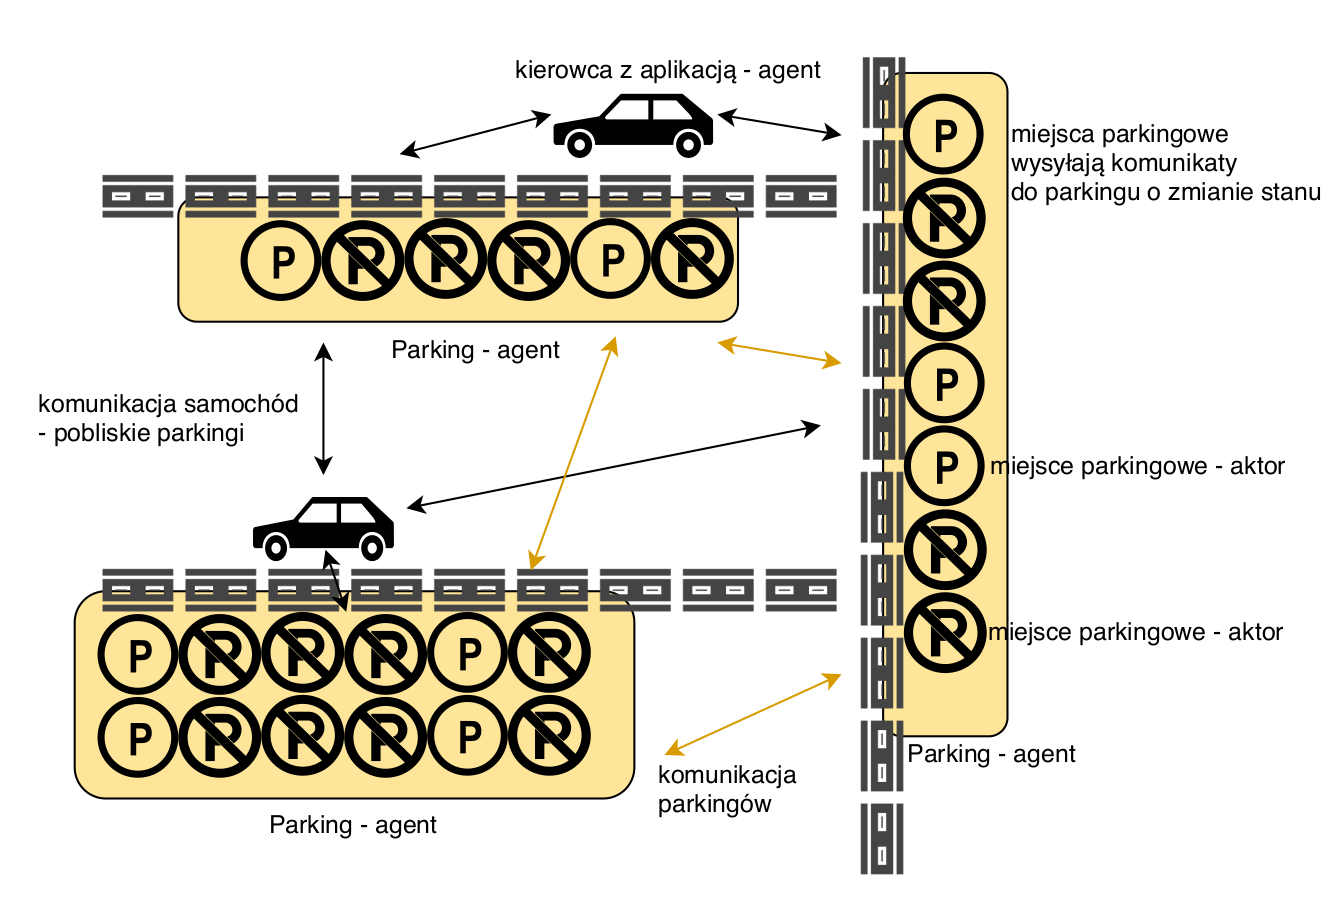
\includegraphics[width=0.8\linewidth]{archi.png}
    \caption{Architektura systemu.}
\end{figure}
\clearpage
\newpage
%--------------------------------------------
% Literatura
%--------------------------------------------


\printbibliography

%--------------------------------------------
% Spisy (opcjonalne)
%--------------------------------------------
\newpage

% Wykaz symboli i skrótów.
% Pamiętaj, żeby posortować symbole alfabetycznie
% we własnym zakresie. Ponieważ mało kto używa takiego wykazu, 
% uznałem, że robienie automatycznie sortowanej listy
% na poziomie LaTeXa to za duży overkill. 
% Jest tylko proste i oczywiste makro \acronym, 
% które dodaje postawowe formatowanie. 
% //AB
% \vspace{0.8cm}
% \section*{Wykaz symboli i skrótów}
% \acronym{EiTI}{Wydział Elektroniki i Technik Informacyjnych}
% \acronym{PW}{Politechnika Warszawska}

\listoffigures              % Spis obrazków. 
\vspace{1cm}                % vertical space
% \listoftables               % Spis tabel. 
% \vspace{1cm}                % vertical space


% \listofappendices           % Spis załączników
% Załączniki
% \appendix

% \newpage
% \newappendix{Nazwa załącznika 1}
% \lipsum[1]

% \newpage
% \newappendix{Nazwa załącznika 2}
% \lipsum[1]

% Używając powyższych spisów jako szablonu,
% możesz tu dodać swój własny wykaz bądź listę, 
% np. spis algorytmów. 

\end{document} % Dobranoc. 

